\documentclass[10pt,a4paper,onecolumn]{article}
\usepackage{marginnote}
\usepackage{graphicx}
\usepackage{xcolor}
\usepackage{authblk,etoolbox}
\usepackage{titlesec}
\usepackage{calc}
\usepackage{tikz}
\usepackage{hyperref}
\hypersetup{colorlinks,breaklinks,
            urlcolor=[rgb]{0.0, 0.5, 1.0},
            linkcolor=[rgb]{0.0, 0.5, 1.0}}
\usepackage{caption}
\usepackage{tcolorbox}
\usepackage{amssymb,amsmath}
\usepackage{ifxetex,ifluatex}
\usepackage{seqsplit}
\usepackage{fixltx2e} % provides \textsubscript
\usepackage[
  backend=biber,
%  style=alphabetic,
%  citestyle=numeric
]{biblatex}
\bibliography{paper.bib}


% --- Page layout -------------------------------------------------------------
\usepackage[top=3.5cm, bottom=3cm, right=1.5cm, left=1.0cm,
            headheight=2.2cm, reversemp, includemp, marginparwidth=4.5cm]{geometry}

% --- Default font ------------------------------------------------------------
% \renewcommand\familydefault{\sfdefault}

% --- Style -------------------------------------------------------------------
\renewcommand{\bibfont}{\small \sffamily}
\renewcommand{\captionfont}{\small\sffamily}
\renewcommand{\captionlabelfont}{\bfseries}

% --- Section/SubSection/SubSubSection ----------------------------------------
\titleformat{\section}
  {\normalfont\sffamily\Large\bfseries}
  {}{0pt}{}
\titleformat{\subsection}
  {\normalfont\sffamily\large\bfseries}
  {}{0pt}{}
\titleformat{\subsubsection}
  {\normalfont\sffamily\bfseries}
  {}{0pt}{}
\titleformat*{\paragraph}
  {\sffamily\normalsize}


% --- Header / Footer ---------------------------------------------------------
\usepackage{fancyhdr}
\pagestyle{fancy}
\fancyhf{}
%\renewcommand{\headrulewidth}{0.50pt}
\renewcommand{\headrulewidth}{0pt}
\fancyhead[L]{\hspace{-0.75cm}\includegraphics[width=5.5cm]{/Library/Frameworks/R.framework/Versions/3.6/Resources/library/rticles/rmarkdown/templates/joss_article/resources/JOSS-logo.png}}
\fancyhead[C]{}
\fancyhead[R]{}
\renewcommand{\footrulewidth}{0.25pt}

\fancyfoot[L]{\footnotesize{\sffamily Sanchez-Reyes et. al., (2020). Physcraper: A Python package for continually updated gene trees. \textit{Journal of Open Source Software}, (), . \href{https://doi.org/}{https://doi.org/}}}


\fancyfoot[R]{\sffamily \thepage}
\makeatletter
\let\ps@plain\ps@fancy
\fancyheadoffset[L]{4.5cm}
\fancyfootoffset[L]{4.5cm}

% --- Macros ---------

\definecolor{linky}{rgb}{0.0, 0.5, 1.0}

\newtcolorbox{repobox}
   {colback=red, colframe=red!75!black,
     boxrule=0.5pt, arc=2pt, left=6pt, right=6pt, top=3pt, bottom=3pt}

\newcommand{\ExternalLink}{%
   \tikz[x=1.2ex, y=1.2ex, baseline=-0.05ex]{%
       \begin{scope}[x=1ex, y=1ex]
           \clip (-0.1,-0.1)
               --++ (-0, 1.2)
               --++ (0.6, 0)
               --++ (0, -0.6)
               --++ (0.6, 0)
               --++ (0, -1);
           \path[draw,
               line width = 0.5,
               rounded corners=0.5]
               (0,0) rectangle (1,1);
       \end{scope}
       \path[draw, line width = 0.5] (0.5, 0.5)
           -- (1, 1);
       \path[draw, line width = 0.5] (0.6, 1)
           -- (1, 1) -- (1, 0.6);
       }
   }

% --- Title / Authors ---------------------------------------------------------
% patch \maketitle so that it doesn't center
\patchcmd{\@maketitle}{center}{flushleft}{}{}
\patchcmd{\@maketitle}{center}{flushleft}{}{}
% patch \maketitle so that the font size for the title is normal
\patchcmd{\@maketitle}{\LARGE}{\LARGE\sffamily}{}{}
% patch the patch by authblk so that the author block is flush left
\def\maketitle{{%
  \renewenvironment{tabular}[2][]
    {\begin{flushleft}}
    {\end{flushleft}}
  \AB@maketitle}}
\makeatletter
\renewcommand\AB@affilsepx{ \protect\Affilfont}
%\renewcommand\AB@affilnote[1]{{\bfseries #1}\hspace{2pt}}
\renewcommand\AB@affilnote[1]{{\bfseries #1}\hspace{3pt}}
\makeatother
\renewcommand\Authfont{\sffamily\bfseries}
\renewcommand\Affilfont{\sffamily\small\mdseries}
\setlength{\affilsep}{1em}


\ifnum 0\ifxetex 1\fi\ifluatex 1\fi=0 % if pdftex
  \usepackage[T1]{fontenc}
  \usepackage[utf8]{inputenc}

\else % if luatex or xelatex
  \ifxetex
    \usepackage{mathspec}
  \else
    \usepackage{fontspec}
  \fi
  \defaultfontfeatures{Ligatures=TeX,Scale=MatchLowercase}

\fi
% use upquote if available, for straight quotes in verbatim environments
\IfFileExists{upquote.sty}{\usepackage{upquote}}{}
% use microtype if available
\IfFileExists{microtype.sty}{%
\usepackage{microtype}
\UseMicrotypeSet[protrusion]{basicmath} % disable protrusion for tt fonts
}{}

\usepackage{hyperref}
\hypersetup{unicode=true,
            pdftitle={Physcraper: A Python package for continually updated gene trees},
            pdfborder={0 0 0},
            breaklinks=true}
\urlstyle{same}  % don't use monospace font for urls
\usepackage{color}
\usepackage{fancyvrb}
\newcommand{\VerbBar}{|}
\newcommand{\VERB}{\Verb[commandchars=\\\{\}]}
\DefineVerbatimEnvironment{Highlighting}{Verbatim}{commandchars=\\\{\}}
% Add ',fontsize=\small' for more characters per line
\usepackage{framed}
\definecolor{shadecolor}{RGB}{248,248,248}
\newenvironment{Shaded}{\begin{snugshade}}{\end{snugshade}}
\newcommand{\AlertTok}[1]{\textcolor[rgb]{0.94,0.16,0.16}{#1}}
\newcommand{\AnnotationTok}[1]{\textcolor[rgb]{0.56,0.35,0.01}{\textbf{\textit{#1}}}}
\newcommand{\AttributeTok}[1]{\textcolor[rgb]{0.77,0.63,0.00}{#1}}
\newcommand{\BaseNTok}[1]{\textcolor[rgb]{0.00,0.00,0.81}{#1}}
\newcommand{\BuiltInTok}[1]{#1}
\newcommand{\CharTok}[1]{\textcolor[rgb]{0.31,0.60,0.02}{#1}}
\newcommand{\CommentTok}[1]{\textcolor[rgb]{0.56,0.35,0.01}{\textit{#1}}}
\newcommand{\CommentVarTok}[1]{\textcolor[rgb]{0.56,0.35,0.01}{\textbf{\textit{#1}}}}
\newcommand{\ConstantTok}[1]{\textcolor[rgb]{0.00,0.00,0.00}{#1}}
\newcommand{\ControlFlowTok}[1]{\textcolor[rgb]{0.13,0.29,0.53}{\textbf{#1}}}
\newcommand{\DataTypeTok}[1]{\textcolor[rgb]{0.13,0.29,0.53}{#1}}
\newcommand{\DecValTok}[1]{\textcolor[rgb]{0.00,0.00,0.81}{#1}}
\newcommand{\DocumentationTok}[1]{\textcolor[rgb]{0.56,0.35,0.01}{\textbf{\textit{#1}}}}
\newcommand{\ErrorTok}[1]{\textcolor[rgb]{0.64,0.00,0.00}{\textbf{#1}}}
\newcommand{\ExtensionTok}[1]{#1}
\newcommand{\FloatTok}[1]{\textcolor[rgb]{0.00,0.00,0.81}{#1}}
\newcommand{\FunctionTok}[1]{\textcolor[rgb]{0.00,0.00,0.00}{#1}}
\newcommand{\ImportTok}[1]{#1}
\newcommand{\InformationTok}[1]{\textcolor[rgb]{0.56,0.35,0.01}{\textbf{\textit{#1}}}}
\newcommand{\KeywordTok}[1]{\textcolor[rgb]{0.13,0.29,0.53}{\textbf{#1}}}
\newcommand{\NormalTok}[1]{#1}
\newcommand{\OperatorTok}[1]{\textcolor[rgb]{0.81,0.36,0.00}{\textbf{#1}}}
\newcommand{\OtherTok}[1]{\textcolor[rgb]{0.56,0.35,0.01}{#1}}
\newcommand{\PreprocessorTok}[1]{\textcolor[rgb]{0.56,0.35,0.01}{\textit{#1}}}
\newcommand{\RegionMarkerTok}[1]{#1}
\newcommand{\SpecialCharTok}[1]{\textcolor[rgb]{0.00,0.00,0.00}{#1}}
\newcommand{\SpecialStringTok}[1]{\textcolor[rgb]{0.31,0.60,0.02}{#1}}
\newcommand{\StringTok}[1]{\textcolor[rgb]{0.31,0.60,0.02}{#1}}
\newcommand{\VariableTok}[1]{\textcolor[rgb]{0.00,0.00,0.00}{#1}}
\newcommand{\VerbatimStringTok}[1]{\textcolor[rgb]{0.31,0.60,0.02}{#1}}
\newcommand{\WarningTok}[1]{\textcolor[rgb]{0.56,0.35,0.01}{\textbf{\textit{#1}}}}
\usepackage{graphicx,grffile}
\makeatletter
\def\maxwidth{\ifdim\Gin@nat@width>\linewidth\linewidth\else\Gin@nat@width\fi}
\def\maxheight{\ifdim\Gin@nat@height>\textheight\textheight\else\Gin@nat@height\fi}
\makeatother
% Scale images if necessary, so that they will not overflow the page
% margins by default, and it is still possible to overwrite the defaults
% using explicit options in \includegraphics[width, height, ...]{}
\setkeys{Gin}{width=\maxwidth,height=\maxheight,keepaspectratio}
\IfFileExists{parskip.sty}{%
\usepackage{parskip}
}{% else
\setlength{\parindent}{0pt}
\setlength{\parskip}{6pt plus 2pt minus 1pt}
}
\setlength{\emergencystretch}{3em}  % prevent overfull lines
\providecommand{\tightlist}{%
  \setlength{\itemsep}{0pt}\setlength{\parskip}{0pt}}
\setcounter{secnumdepth}{0}
% Redefines (sub)paragraphs to behave more like sections
\ifx\paragraph\undefined\else
\let\oldparagraph\paragraph
\renewcommand{\paragraph}[1]{\oldparagraph{#1}\mbox{}}
\fi
\ifx\subparagraph\undefined\else
\let\oldsubparagraph\subparagraph
\renewcommand{\subparagraph}[1]{\oldsubparagraph{#1}\mbox{}}
\fi



\title{Physcraper: A Python package for continually updated gene trees}

        \author[1]{Luna L. Sanchez Reyes}
          \author[1]{Emily Jane McTavish}
    
      \affil[1]{University of California, Merced}
      \affil[2]{Institution 2}
  \date{\vspace{-5ex}}

\begin{document}
\maketitle

\marginpar{
  %\hrule
  \sffamily\small

  {\bfseries DOI:} \href{https://doi.org/}{\color{linky}{}}

  \vspace{2mm}

  {\bfseries Software}
  \begin{itemize}
    \setlength\itemsep{0em}
    \item \href{}{\color{linky}{Review}} \ExternalLink
    \item \href{}{\color{linky}{Repository}} \ExternalLink
    \item \href{}{\color{linky}{Archive}} \ExternalLink
  \end{itemize}

  \vspace{2mm}

  {\bfseries Submitted:} \\
  {\bfseries Published:} 

  \vspace{2mm}
  {\bfseries License}\\
  Authors of papers retain copyright and release the work under a Creative Commons Attribution 4.0 International License (\href{http://creativecommons.org/licenses/by/4.0/}{\color{linky}{CC-BY}}).
}

\hypertarget{summary}{%
\section{Summary}\label{summary}}

\begin{enumerate}
\def\labelenumi{\arabic{enumi}.}
\item
  Phylogenies are still a key part of research in all areas of biology.
  The nonspecialist can use one of the many tools available to
  automatize phylogenetic reconstruction. However, interpretation of
  results, comparison with previously available phylogenetic hypotheses,
  and choosing of one phylogeny for discussion still impose difficulties
  to one that is not a specialist on phylogenetic methods or on a
  particular group of study.
\item
  Physcraper is an open‐source Python program that automatizes the
  update of public phylogenies by making use of public DNA sequence data
  and taxonomic information.
\item
  Physcraper can be used by the nonspecialist, as a tool to generate
  phylogenetic hypothesis based on public expert phylogentic knowledge.
  The phylogenetics and group specialist will find it useful as a tool
  to facilitate comparison of alternative phylogenetic hypotheses
  (topologies). \textbf{\emph{Is physcraper intended for the
  nonspecialist?? We have two types of nonspecialists: the ones that do
  not know about phylogenetic methods and the ones that might know about
  phylogenetic methods but do not know of a certain biological group.}}
\item
  Physcraper implements node by node comparison of the the original and
  the updated trees using the conflict API of OToL.
\item
  We hope the physcraper workflow demonstrates the benefits of open
  results in phylogenetics and encourages researchers to strive for
  better data sharing practices.
\item
  Physcraper can be used with any OS. Detailed instructions for
  installation and use are available at
  \url{https://github.com/McTavishLab/physcraper}.
\end{enumerate}

\hypertarget{intro}{%
\section{Intro}\label{intro}}

There is a lot of phylogenetic knowledge already available. Some of it
has been made public at OToL. Most or all public phylogenies have the
potential to be updated with the ever increasing amount of genetic data
that is available on GenBank. There are now various methods to
automatize use of GenBank data for phylogenetic reconstruction, which
are generally intended to facilitate the use of phylogenetic knowledge
for the nonspecialist. However, none of them provide a means to compare
with previously available expert knowledge on a particular group.

A key aspect of the standard phylogenetic workflow is comparison with
already existing phylogenetic hypotheses and with phylogenies that are
considered ``best'' by experts not only in phylogenetics, but also
experts of the focal group of study.

It is well known that GenBank holds enormous amounts of genetic data,
and it continues to grow. A lot of this genetic data has the potential
to be used to reconstruct the phylogenetic history of various organisms
(Sanderson, Boss, Chen, Cranston, \& Wehe, 2008). Pipelines that harness
this potential have been available for over a decade now, such as the
Phylota brower, and PHLAWD. New ones keep on being developed, such as
SUPERSMART and the upgraded version of PHLAWD, PyPHLAWD. Notably large
phylogenies have been constructed using some of these tools, Some other
have not been used that much. So, how well accepted is this approach in
the community?

Concerns with these tools: Errors in identification of sequences Little
control along the process Too much of a black box?

Most of these phylogenies are being constructed by people learning about
the methods, so they want to know what is going on.

The pipelines are so powerful and they will give you an answer, but
there is no way to assess if it is better than previous answers, it just
assumes it is better because it used more data.

All these pipelines start tree consruction from zero?

The goal of Physcraper is to build upon previous phylogenetic knowledge,
allowing a direct comparison of existing phylogenies to phylogenies that
are constructed using new genetic data from GenBank

To achieve this, Physcraper uses the Open Tree of Life phylesystem and
connects it to the TreeBase database, to (1) get the original DNA
dataset matrices (alignments) that produced a phylogeny that was
published and then made available in the OToL database, (2) use this DNA
alignments as a starting point to get new genetic data belonging to the
focal group of study, to (3) finally update the phylogenetic
relationships in the group.

A less automated workflow is one in which the alignments that generated
the published phylogeny are stored in other public database (such as
DRYAD) or elsewhere (the users computer), and are provided by the users.

The original tree is by defualt used as starting tree for the
phylogenetic searches, but it can also be set as a full topological
constraint or not used at all, depending on the goals of the user.

Physcraper implements node by node comparison of the the original and
the updated trees, using the conflict API of OToL.

\hypertarget{physcraper-overview}{%
\section{Physcraper overview}\label{physcraper-overview}}

\hypertarget{examples}{%
\section{Examples}\label{examples}}

Imagine you are starting to work on a new biological group X. You have
not much of an idea about its phylogenetic relationships, you are a
newly established researcher, and the group is not anything any of your
collaborators have worked on before. A good idea is to start an
intensive litt review on the phylogenetics of the group. Rapidly, you
find out there are 5 different phylogeneis, that used different markers,
and that the papers, published at different times, do not discuss which
phylogeny is the one accepted by the expert community on X. You might
need to go to the annual conference of X, and even then, you might only
find different and contrasting opinions. Somewhere along these months or
even years doing this task, you looked into the the OToL database. You
found in there some or all the published trees of X, along with a tree
that has been deemed the best tree by curators and ideally experts on X?

Let's be more specific now about our X group and say it is the
Ascomycota. The best tree currently available in OToL was published by
Schoch et al. (2009). The first step, is to get the Open Tree of Life
study id. There are some options to do this: - You can go to the Open
Tree of Life website and browse until you find it, or - you can get the
study id using R tools: - By using the treebase ID of the study (which
is not fully exposed on the Treebase website home page of the study, so
you have to really look it up manually):

\begin{Shaded}
\begin{Highlighting}[]
\NormalTok{rotl}\OperatorTok{::}\KeywordTok{studies_find_studies}\NormalTok{(}\DataTypeTok{property =} \StringTok{"treebaseId"}\NormalTok{, }\DataTypeTok{value =} \StringTok{"S2137"}\NormalTok{)}
\CommentTok{##   study_ids n_trees         tree_ids candidate study_year title}
\CommentTok{## 1    pg_238       2 tree109, tree110                 2009      }
\CommentTok{##                                 study_doi}
\CommentTok{## 1 http://dx.doi.org/10.1093/sysbio/syp020}
\end{Highlighting}
\end{Shaded}

\begin{itemize}
\tightlist
\item
  By using the name of the focal clade of study (but this behaved very
  differently):
\end{itemize}

\begin{Shaded}
\begin{Highlighting}[]
\NormalTok{rotl}\OperatorTok{::}\KeywordTok{studies_find_studies}\NormalTok{(}\DataTypeTok{property=}\StringTok{"ot:focalCladeOTTTaxonName"}\NormalTok{, }\DataTypeTok{value=}\StringTok{"Ascomycota"}\NormalTok{)}
\end{Highlighting}
\end{Shaded}

Once we have the study id, we can gather the trees published on that
study:

\begin{Shaded}
\begin{Highlighting}[]
\NormalTok{rotl}\OperatorTok{::}\KeywordTok{get_tree_ids}\NormalTok{(rotl}\OperatorTok{::}\KeywordTok{get_study_meta}\NormalTok{(}\StringTok{"pg_238"}\NormalTok{))}
\CommentTok{## [1] "tree109" "tree110"}
\NormalTok{rotl}\OperatorTok{::}\KeywordTok{candidate_for_synth}\NormalTok{(rotl}\OperatorTok{::}\KeywordTok{get_study_meta}\NormalTok{(}\StringTok{"pg_238"}\NormalTok{))}
\CommentTok{## NULL}
\NormalTok{my_trees <-}\StringTok{ }\NormalTok{rotl}\OperatorTok{::}\KeywordTok{get_study}\NormalTok{(}\StringTok{"pg_238"}\NormalTok{)}
\end{Highlighting}
\end{Shaded}

Both trees from this study have 434 tips.

Let's check what one of the trees looks like:

\begin{Shaded}
\begin{Highlighting}[]
\NormalTok{ape}\OperatorTok{::}\KeywordTok{plot.phylo}\NormalTok{(my_trees[[}\DecValTok{1}\NormalTok{]], }\DataTypeTok{type =} \StringTok{"fan"}\NormalTok{)}
\end{Highlighting}
\end{Shaded}

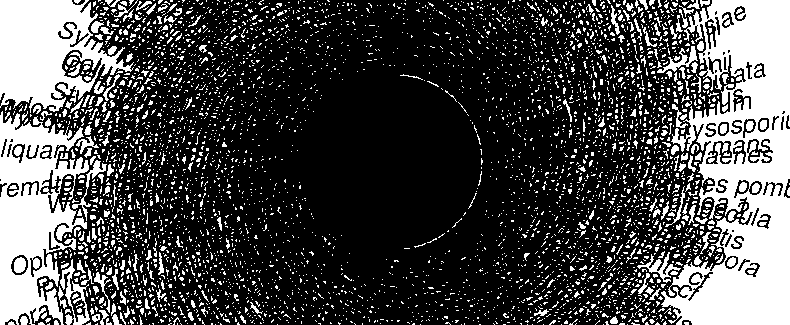
\includegraphics[width=468px]{physcraper_ms_ 2020-05-05_files/figure-latex/fungi-phylo-1}

\begin{enumerate}
\def\labelenumi{\arabic{enumi}.}
\tightlist
\item
  Download the alignment from Treebase If you are on the Treebase home
  page of the study, you can navigate to the matrix tab, and manually
  download the alignments that were used to reconstruct the trees
  reported on the study that were also uploaded to Treebase and to the
  Open Tree of Life repository. To make this task easier, you can use a
  command to download everything into your working folder:
\end{enumerate}

\begin{verbatim}
physcraper_run.py -s pg_238 -t tree109 -o ../physcraper_example/pg_238
\end{verbatim}

In this example, all alignments posted on Treebase were used to
reconstruct both trees.

\begin{enumerate}
\def\labelenumi{\arabic{enumi}.}
\tightlist
\item
  With the study id and the alignment files saved locally, we can do a
  physcraper run with the command:
\end{enumerate}

\begin{verbatim}
physcraper_run.py -s pg_238 -t tree109 -a treebase_alns/pg_238tree109.aln -as "nexus" -o pg_238
\end{verbatim}

\hypertarget{tools-on-a-similar-track}{%
\section{Tools on a similar track:}\label{tools-on-a-similar-track}}

Tools that do similar things: pyPhlawd (Smith \& Walker, 2019)
SUPERSMART (Antonelli et al., 2017)

\hypertarget{acknowledgements}{%
\section{Acknowledgements}\label{acknowledgements}}

We acknowledge contributions from

\hypertarget{references}{%
\section*{References}\label{references}}
\addcontentsline{toc}{section}{References}

\hypertarget{refs}{}
\leavevmode\hypertarget{ref-antonelli2017toward}{}%
Antonelli, A., Hettling, H., Condamine, F. L., Vos, K., Nilsson, R. H.,
Sanderson, M. J., Sauquet, H., et al. (2017). Toward a self-updating
platform for estimating rates of speciation and migration, ages, and
relationships of taxa. \emph{Systematic Biology}, \emph{66}(2),
152--166.

\leavevmode\hypertarget{ref-sanderson2008phylota}{}%
Sanderson, M. J., Boss, D., Chen, D., Cranston, K. A., \& Wehe, A.
(2008). The PhyLoTA Browser: Processing GenBank for Molecular
Phylogenetics Research. \emph{Systematic Biology}, \emph{57}(3),
335--346.
doi:\href{https://doi.org/10.1080/10635150802158688}{10.1080/10635150802158688}

\leavevmode\hypertarget{ref-schoch2009ascomycota}{}%
Schoch, C. L., Sung, G.-H., López-Giráldez, F., Townsend, J. P.,
Miadlikowska, J., Hofstetter, V., Robbertse, B., et al. (2009). The
ascomycota tree of life: A phylum-wide phylogeny clarifies the origin
and evolution of fundamental reproductive and ecological traits.
\emph{Systematic biology}, \emph{58}(2), 224--239.

\leavevmode\hypertarget{ref-smith2019pyphlawd}{}%
Smith, S. A., \& Walker, J. F. (2019). PyPHLAWD: A python tool for
phylogenetic dataset construction. \emph{Methods in Ecology and
Evolution}, \emph{10}(1), 104--108.

\end{document}
